% !TEX program = pdflatex
% !TEX encoding = UTF-8
% !TEX spellcheck = en_US

\documentclass[11pt, a4paper, notitlepage]{article}

\usepackage{settings}

\geometry{margin=1cm}
\graphicspath{./}
\addbibresource[label=main]{./publications.bib}


%---------------------------------------------------------------------------------------------------------------------------------------------
%				DOCUMENT
%---------------------------------------------------------------------------------------------------------------------------------------------
\begin{document}
\fontencoding{T2A}\selectfont
\pagestyle{empty}
%---------------------------------------- SERBIAN VERSION ---------------------------------------------------
	\newpage
	\selectlanguage{serbian}

	\cvname{Милан Скочић, \keeplatin{PhD}}
	
	\cvjob{Електрохемија и Материјали}
	
	\cvinfo{milan.skocic@icloud.com}
	{+33(0)6 66 18 69}
	{github.com/MilanSkocic}
	{2500C Route de Saint Sernin, 71200 Saint Sernin du Bois, France}
	{0000-0003-2189-5766}

	%----------------------------------------------------------------------------------------------
	\section*{Радно искуство}

	\cventry{Мај 2017}{Данас}{\keeplatin{PhD}, електрохемичар}{\keeplatin{Framatome}}{Француска}
	\begin{jobdetails}[T2A]
		\item Пројектни менаџмент
 		\item Електрохемија на високим температурама
		\item Корозија легура од \keeplatin{Zr} и \keeplatin{Ni} у воденој средини на високим температурама
	\end{jobdetails}
		
	\cventry{Окт. 2015}{Март 2017}{\keeplatin{PhD}, металних материјала}{\keeplatin{Areva NP}}{Француска}
	\begin{jobdetails}[T2A]
		\item Пројектни менаџмент
		\item Напонска корозија \keeplatin{Inconel 718}
		\item Корозија легура од цирконијума
	\end{jobdetails}

    \cventry{Окт. 2012}{Окт. 2015}{\keeplatin{PhD} пројекат - "Фото-електрохемијско истраживање \keeplatin{Shadow} корозије"}{\keeplatin{Areva/SIMaP Lab.}}{Француска}
	\begin{jobdetails}[T2A]
		\item Пројектни менаџмент и реализација нове електрохемијске ћелије за тестирање корозије на високој температури и на високом притиску
		\item Оверавање нове електрохемијске ћелиjе
		\item (Фото-)електрохемијске карактеризациje на високој температури и на високом притиску
		\item Свакодневни тестови у аутоклавима на високој температури и на високом притиску
		\item Купловање са петљом за контролу хемије
	\end{jobdetails}
	
	\cventry{Fеб. 2012}{Aвг. 2012}{\keeplatin{Master} - "Металне плоче за горивне ћелиjе \keeplatin{PEM}"}{\keeplatin{Air Liquide}}{Француска}
	\begin{jobdetails}[T2A]
		\item Стање уметности о обложеним нерђајућим челицима – Успоставио електрохемијске тестове
		\item Мерио отпор граничне површине
		\item Посматрање \keeplatin{TEM/SEM}
	\end{jobdetails}

	\cventry{Aпр. 2011}{Aвг. 2011}{\keeplatin{Master} асистент - "Композицијски разврстани челици"}{Факултет \keeplatin{McMaster}, Одељење за инжењеринг материjала}{Канада}
	\begin{jobdetails}[T2A]
		\item Цементациjа
		\item Припремао примерке квантификовао размеру фаза у микроструктурама
		\item Моделовање номиналног напона под компресијом
	\end{jobdetails}

	\cventry{2007}{2009}{Техничар}{\keeplatin{ArcelorMittal R\&D center}}{Француска}
	\begin{jobdetails}[T2A]
		\item Припремао примерке: сечење, опточење, полирање
		\item Изводио микроструктуралне анализе: \keeplatin{SEM}, \keeplatin{TEM}, рендгенска кристалографија
		\item Изводио термо-механичке третмане: \keeplatin{Gleeble}, топло ваљање, тест затезања
	\end{jobdetails}

	\cventry{Aвг. 2005}{Jун. 2006}{Техничар}{Центар за пиролизу (\keeplatin{CPM})}{Француска}
	\begin{jobdetails}[T2A]
		\item Учествовао у истраживањима са коксаном пећи
		\item Припремао и извршавао тестове на разне врсте угља и кокса
	\end{jobdetails}
	
	\newpage
        %------------------------------------------------------------------------------------------------
	\section*{Образовање}
	\cvedentry{2012}{2015}{Доктор, Материјали и Електрохемија}{Доксторски колеџ у Греноблу}{Француска}
	
	\cvedentry{2009}{2012}{Инжењер, Електрохемија}{Факултет у Греноблу (\keeplatin{PHELMA})}{Француска}

	\cvedentry{2003}{2005}{Техничар, Аналитичка Хемиjа}{Факултет у Мецу}{Француска}

	%----------------------------------------------------------------------------------------------
	\section*{Језици}
	Српски \faStar\faStar\faStar\faStar\faStar \hfill
    	Француски \faStar\faStar\faStar\faStar\faStar \hfill
    	Енглески \faStar\faStar\faStar\faStar\faStarO

	%----------------------------------------------------------------------------------------------
	\section*{Комјутерске вештине}
	{\fontencoding{T1}\selectfont\
	\begin{center}
	    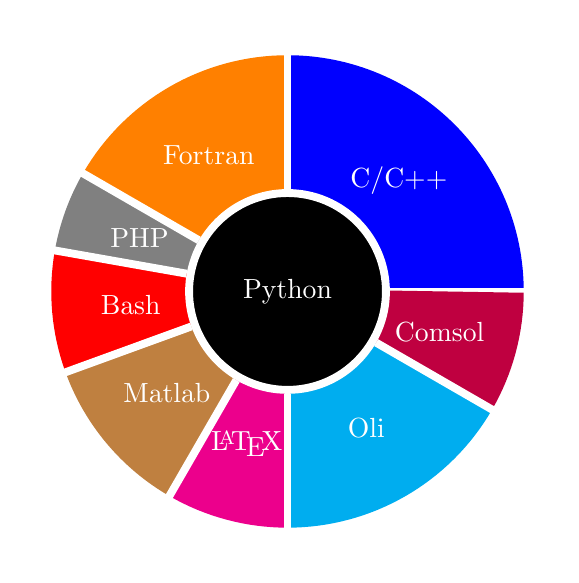
\begin{tikzpicture}[text=white, border/.style={line width=20mm}]
		\foreach \angle/\col [remember=\angle as \last (initially 0)] 
		    in {90/blue, 150/orange, 170/gray, 200/red, 240/brown, 270/magenta, 330/cyan, 360/purple}{
			\draw[\col, border] (\last:2cm) arc[start angle=\last, end angle=\angle, radius=2cm];
			\draw[white, line width=1mm] (\last:1.3)--++(\last:2.0);}
			\node[line width=1mm, draw, circle, minimum width=2.5cm, white, fill=black]{Python};
			\node at (45:2cm) {C/C++};
			\node at (120:2cm) {Fortran};
			\node at (160:2cm) {PHP};
			\node at (185:2cm) {Bash};
			\node at (220:2cm) {Matlab};
			\node at (255:2cm) {\LaTeX};
			\node at (300:2cm) {Oli};
			\node at (345:2cm) {Comsol};

	    \end{tikzpicture}
	\end{center}}

    %----------------------------------------------------------------------------------------------
    \section*{\keeplatin{PhDs} - Техничка подршка}

    \href{https://tel.archives-ouvertes.fr/tel-02304680/}{\keeplatin{S. El Euch, “Recherche d’une corrélation entre caractéristiques électrochimiques et relâchement en nickel de l’alliage 690 en milieu primaire d’un réacteur à eau pressurisée,” Université Sorbonne, Paris, 2019.}}
 	
    \href{http://www.theses.fr/s222058}{\keeplatin{F. Da Fonseca, “Etude du phénomène de shadow corrosion des alliages de zirconium dans les réacteurs à eau bouillante (REB),” Université de Grenoble Alpes, Grenoble, 2021.}}


    \href{http://www.theses.fr/s217506}{\keeplatin{J. Ben Mohamed, “Etude des mécanismes de Corrosion sous contrainte des alliages 600/690 en milieu secondaire des réacteurs REP en présence de plomb et de soufre.,” Ecole Nationale Supérieure des Mines de Saint-Etienne, Saint-Etienne, 2021.}}
    
    \href{http://www.theses.fr/s278984}{\keeplatin{D. Peyret, “Mécanismes électrochimiques de la corrosion des alliages de type ZrNbX en condition simulées de réacteur à eau pressurisée,” Université Sorbonne, Paris, 2023.}}
	
    %----------------------------------------------------------------------------------------------
	\newpage
	\nocite{*}
	\printbibliography[title=Публикације]
\end{document}
